\subsection{Set point Weights}
        Mit den set point weights kann das Regelverhalten verbessert werden. Dabei wird die Referenz $r(t)$ seperat mit einer Verstärkung ($a,\, b,\, c$) multipliziert.
        
        \begin{figure}[H]
            \centering
            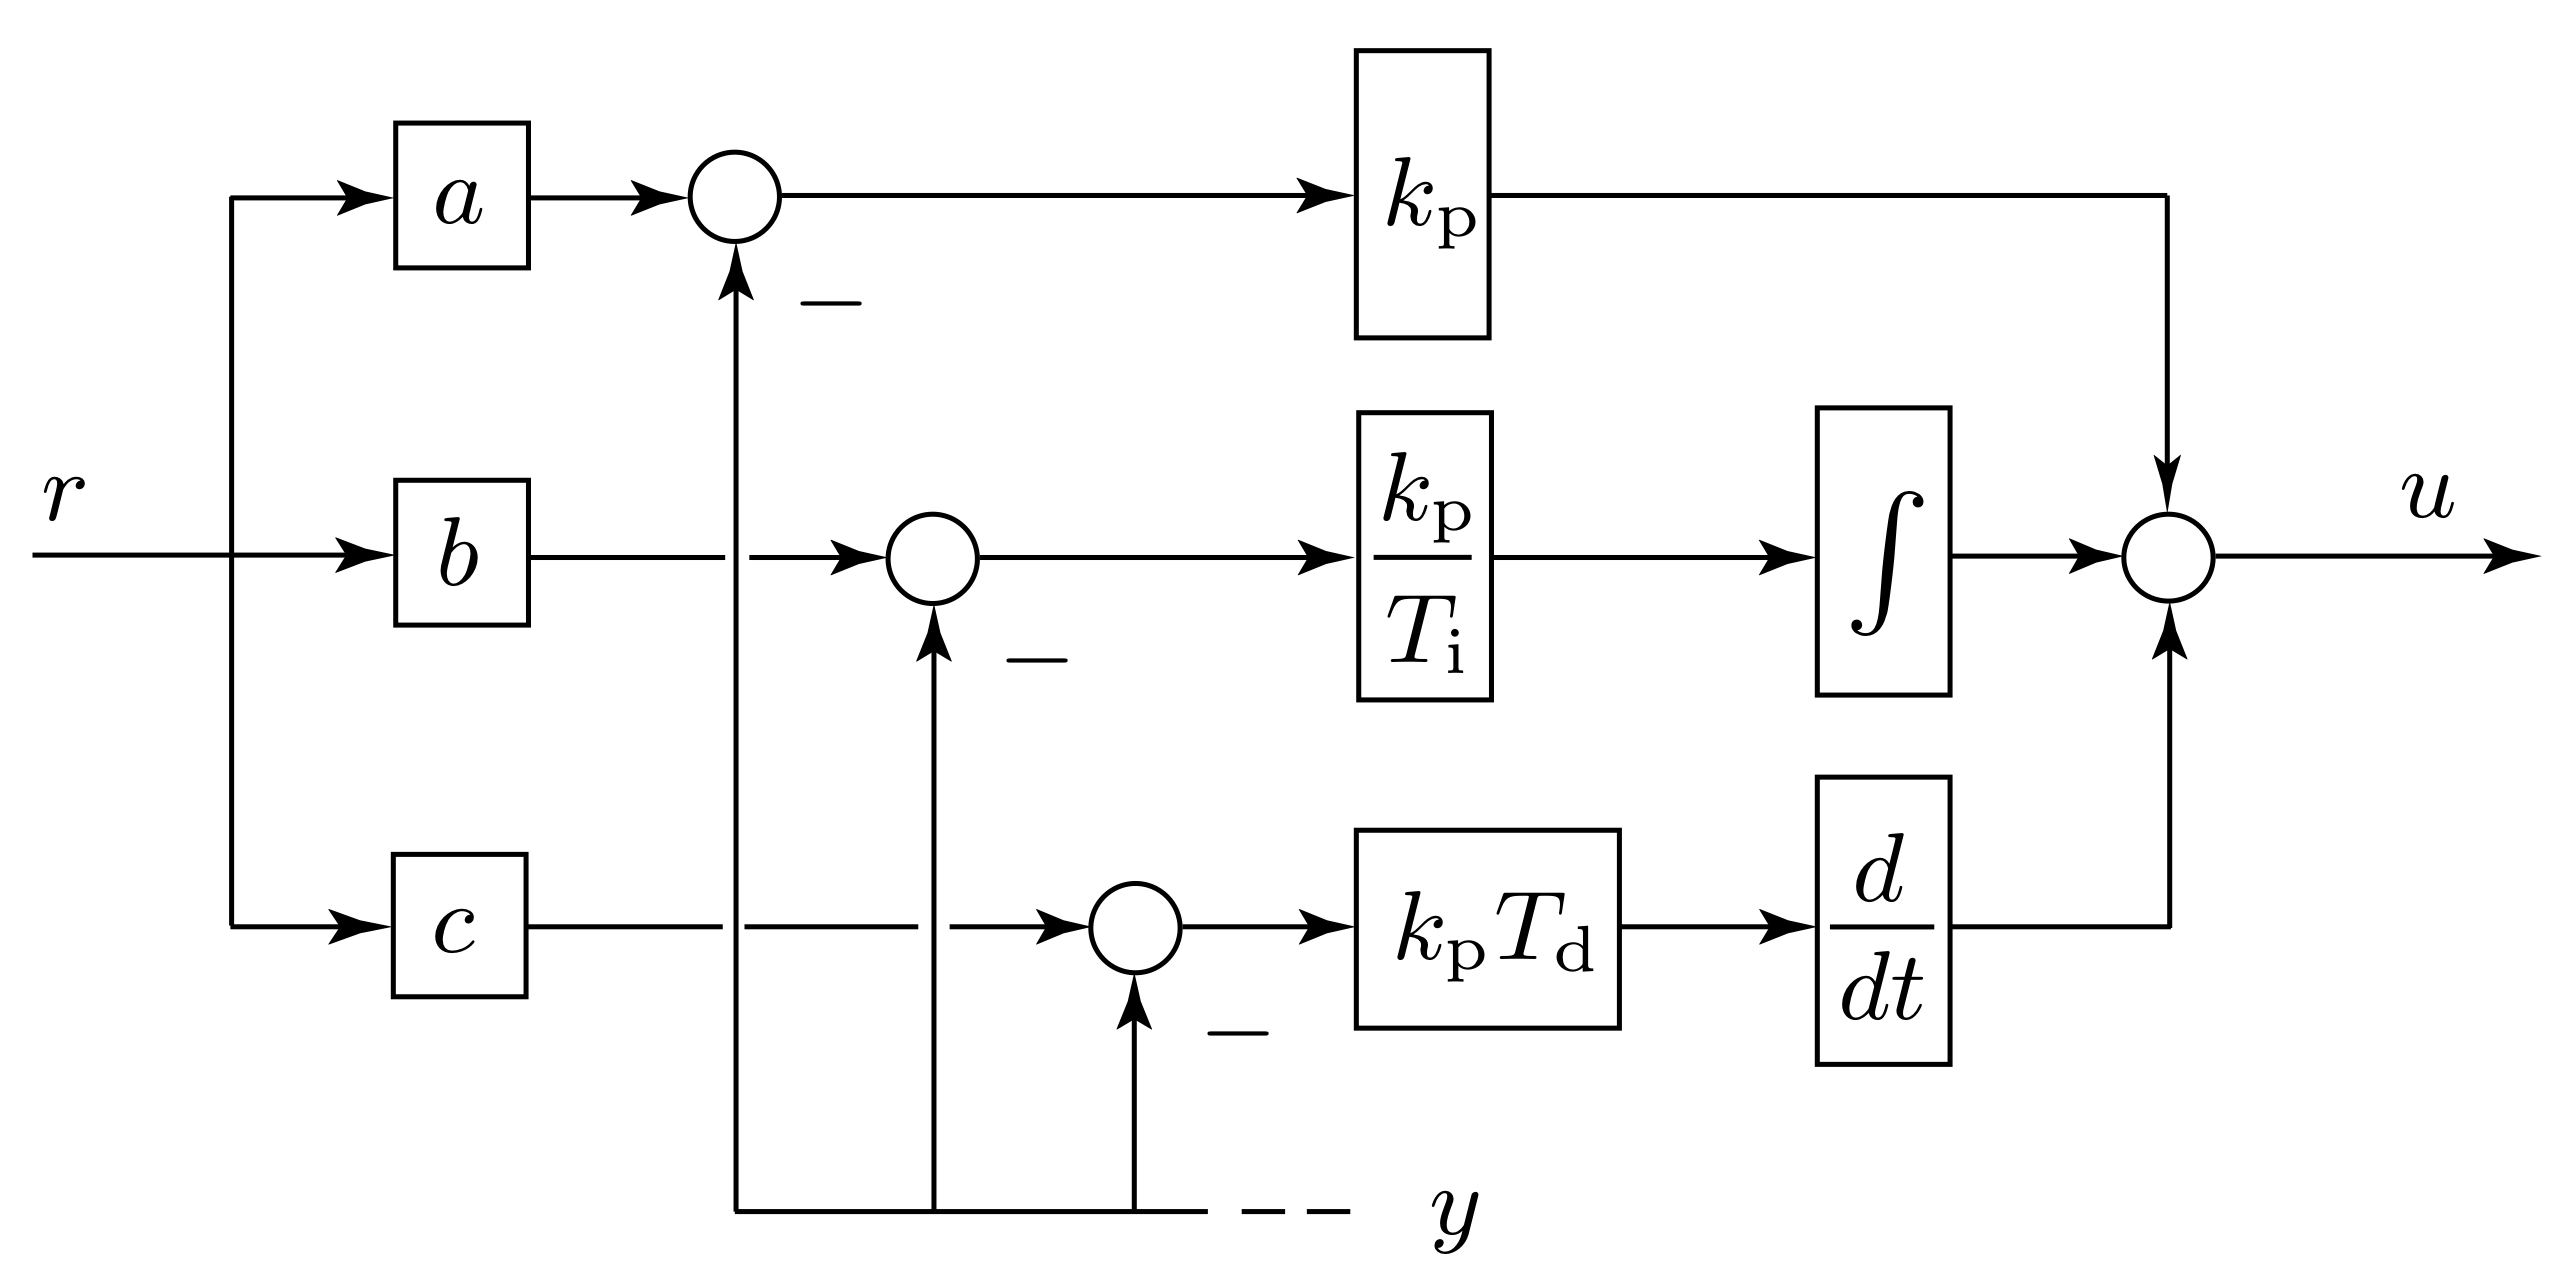
\includegraphics[width = 0.535\linewidth]{images/04/spw.jpeg}
        \end{figure}
        
        \begin{itemize}
            \item $b=1$ um einen statischen Nachlauffehler zu verhindern falls die Referenz möglichst konstant werden soll.
            
            \item $c=0$ Normalerweise will man nur Änderungen aufgrund des Ausgangssignals dämpfen. Ein Step in $r(t)$ würde auf dem Differential-Pfad zu einem Dirac-Stoss führen.
            
            \item $a$ wird mit \r{A}ström-Hägglund bestimmt. Typischerweise wählt man $a\in(0,1)$. Ein guter Wert für $a$ verbesert häufig das closed-loop Verhalten.
        \end{itemize}
        \textbf{Bemerkung:} Die Gewichtungen Beeinflussen die Stabilität des geschlossenen Reglekreises \textbf{nicht!}
        \begin{equation*}
            T(s) = \frac{Y(s)}{R(s)}\frac{P\cdot\overbrace{\Big(a\cdot k_p +b\cdot\frac{k_p}{T_i\cdot s} + c\cdot k_p\cdot T_d\cdot s\big)}^{C_{\textnormal{PID,weighted}}}}{1 + P\cdot\underbrace{\Big(k_p + \frac{k_p}{T_i\cdot s} + k_p\cdot T_d\cdot s\big)}_{C_{\textnormal{PID,unweighted}}}}
        \end{equation*}